\begin{figure}[h]
	\centering
	\setlength{\resLen}{3.in}
	\setlength{\raiseLen}{0.3in}	
	\addtolength{\tabcolsep}{-3pt}
	\begin{tabular}{c @{\hspace{2\tabcolsep}} ccc}
		\raisebox{\raiseLen}{\rotatebox[origin=c]{90}{GT}} &
		\includegraphics[width=\resLen]{svbrdf/validation/embed/fake_018/tex_ref.jpg} & &
		\includegraphics[width=\resLen]{svbrdf/validation/embed/fake_037/tex_ref.jpg}
		\\
		\raisebox{\raiseLen}{\rotatebox[origin=c]{90}{$\calW$}} & 
		\includegraphics[width=\resLen]{svbrdf/validation/embed/fake_018/tex_W.jpg} & &
		\includegraphics[width=\resLen]{svbrdf/validation/embed/fake_037/tex_W.jpg}
		\\
		\raisebox{\raiseLen}{\rotatebox[origin=c]{90}{$\calW^+$}} &
		\includegraphics[width=\resLen]{svbrdf/validation/embed/fake_018/tex_W+.jpg} & &
		\includegraphics[width=\resLen]{svbrdf/validation/embed/fake_037/tex_W+.jpg}
		\\
		\raisebox{\raiseLen}{\rotatebox[origin=c]{90}{$\calWN$}} &
		\includegraphics[width=\resLen]{svbrdf/validation/embed/fake_018/tex_W+N.jpg} & &
		\includegraphics[width=\resLen]{svbrdf/validation/embed/fake_037/tex_W+N.jpg}
	\end{tabular}
	\caption[Embedding SVBRDFs into different latent spaces]{\label{fig:svbrdf:embed}
		\textbf{Embedding SVBRDFs into different latent spaces.} We take two synthetic SVBRDF material maps (top) and embed them into different latent spaces with and without the noise space (second--fourth rows). For illustration, we also embed the maps into a pure-noise space \emph{only}; this is unable to recover the color at all.
	}
\end{figure}